%%%%%%%%%%%%%%%%%%%%%%%%%%%%%%%%%%%%%%%%%
% Large Colored Title Article
% LaTeX Template
% Version 1.1 (25/11/12)
%
% This template has been downloaded from:
% http://www.LaTeXTemplates.com
%
% Original author:
% Frits Wenneker (http://www.howtotex.com)
%
% License:
% CC BY-NC-SA 3.0 (http://creativecommons.org/licenses/by-nc-sa/3.0/)
%
%%%%%%%%%%%%%%%%%%%%%%%%%%%%%%%%%%%%%%%%%

%----------------------------------------------------------------------------------------
%	PACKAGES AND OTHER DOCUMENT CONFIGURATIONS
%----------------------------------------------------------------------------------------

\documentclass[DIV=calc, paper=a4, fontsize=11pt,twocolumn,margin=.5in]{scrartcl}	 % A4 paper and 11pt font size

\usepackage{lipsum} % Used for inserting dummy 'Lorem ipsum' text into the template
\usepackage[english]{babel} % English language/hyphenation
\usepackage[protrusion=true,expansion=true]{microtype} % Better typography
\usepackage{amsmath,amsfonts,amsthm} % Math packages
\usepackage[svgnames]{xcolor} % Enabling colors by their 'svgnames'
\usepackage[font=small,labelfont=bf, justification=justified,format=plain]{caption}
\usepackage{booktabs} % Horizontal rules in tables
\usepackage{fix-cm}	 % Custom font sizes - used for the initial letter in the document
\usepackage{soul}
\usepackage{graphicx}
\usepackage{color}
\usepackage[numbers]{natbib}
\usepackage{fancyhdr}
\usepackage[export]{adjustbox}
\usepackage{wrapfig}
\bibliographystyle{abbrv}
%\usepackage{helvet}
%\renewcommand{\familydefault}{\sfdefault}


\usepackage{titlesec}

\usepackage{sectsty} % Enables custom section titles
\allsectionsfont{\color{DarkGoldenrod}\usefont{OT1}{phv}{b}{n}} % Change the font of all section commands

\usepackage{fancyhdr} % Needed to define custom headers/footers
\pagestyle{fancy} % Enables the custom headers/footers
\fancyhf{}

\usepackage{lastpage} % Used to determine the number of pages in the document (for "Page X of Total")

% Headers - all currently empty
\lhead{}
\chead{}
\rhead{}

% Footers
\lfoot{ \includegraphics[scale=0.15,valign=c]{iic.jpg}
               \includegraphics[scale=0.32,valign=c]{harris.png}
              \includegraphics[scale=0.15,valign=c]{ipam.png}
              \includegraphics[scale=0.1,valign=c]{usaid.png}
              \includegraphics[scale=0.23,valign=c]{whrc.png}  
              \includegraphics[scale=0.23,valign=c]{mbl.jpg}           
            }


\renewcommand{\headrulewidth}{0.0pt} % No header rule
\renewcommand{\footrulewidth}{0.4pt} % Thin footer rule

\usepackage{lettrine} % Package to accentuate the first letter of the text
\newcommand{\initial}[1]{ % Defines the command and style for the first letter
\lettrine[lines=3,lhang=0.3,nindent=0em]{
\color{DarkGoldenrod}
{\textsf{#1}}}{}}

%----------------------------------------------------------------------------------------
%	TITLE SECTION
%----------------------------------------------------------------------------------------

\usepackage{titling} % Allows custom title configuration

\newcommand{\HorRule}{\color{DarkGoldenrod} \rule{\linewidth}{1pt} \hrule\vspace{-2em}} % Defines the gold horizontal rule around the title


\pretitle{\vspace{-30pt} \begin{flushleft} \HorRule \fontsize{20}{20} \usefont{OT1}{phv}{b}{n} \color{DarkGreen} \selectfont} % Horizontal rule before the title

\title{{\color{black}IIC Brazil Summer Policy Lab}\\ \vspace{.3cm}Constru\c c\~{a}o de Hidrel\'{e}tricas e Desmatamento: Relacionando Cobertura Florestal com Mudan\c cas no Balan\c co H\'{i}drico} % Your article title

\posttitle{\par\end{flushleft}\vskip 0.5em \vspace{-1.5em}} % Whitespace under the title

\preauthor{\begin{flushleft}\large \lineskip 0.5em \usefont{OT1}{phv}{b}{sl} \color{DarkGreen}} % Author font configuration
\author{Soudeep Deb\textsuperscript{1}, Joel Smith\textsuperscript{2}, Ane Alencar\textsuperscript{3}, Isabel Silva\textsuperscript{3} and Michael Coe\textsuperscript{4}\\} % Your name

\postauthor{\footnotesize \usefont{OT1}{phv}{m}{sl} \color{Black} % Configuration for the institution name
\textsuperscript{1}Department of Statistics, University of Chicago, Chicago, IL, USA; sdeb@uchicago.edu\\
\textsuperscript{2}Department of Ecology and Evolution, University of Chicago, Chicago, IL, USA; joelsmith@uchicago.edu\\
\textsuperscript{3}Instituto de Pesquisa Ambiental do Amaz\^ onia, Bras\'{i}lia, Brasil\\
\textsuperscript{4}Woods Hole Research Center, Falmouth, MA, USA
\vspace{-2em}
\par\end{flushleft}\HorRule} % Horizontal rule after the title
\date{} % Add a date here if you would like one to appear underneath the title block
\renewcommand{\figurename}{Fig.}
\addto\captionsenglish{\renewcommand{\figurename}{Figura}}

%----------------------------------------------------------------------------------------t

\begin{document}

\maketitle % Print the title
\thispagestyle{fancy} % Enabling the custom headers/footers for the first page 
\initial{A} constru\c c\~{a}o de usinas hidrel\'{e}tricas representa o maior vetor potencial de desmatamento na Amaz\^ onia como resultado de: (1) constru\c c\~{a}o de estradas de acesso para \'{a}reas remotas; (2) migra\c c\~{a}o trabalhadores que geram um r\'{a}pido aumento na densidade populacional; e (3) a constru\c c\~{a}o da infraestrutura necess\'{a}ria para suportar esse crescimento populacional. Em novembro de 2015, 237 barragens haviam sido planejadas ou estavam em constru\c c\~{a}o na Amaz\^ onia brasileira \cite{castello2015large}. A constru\c c\~{a}o de hidrel\'{e}tricas na Bacia do Rio Tapaj\'{o}s representou um ter\c co desse total. A quantidade estimada de \'{a}rea total desmatada at\'{e} 2030 na Bacia do Rio Tapaj\'{o}s ser\'{a} 42\% a 105\% maior do que o esperado sem a constru\c c\~{a}o de hidrel\'{e}tricas (Fig. 1). No in\'{i}cio de Agosto de 2016, a licen\c ca ambiental para construir a maior dentre essas barragens, a S\~{a}o Luiz do Tapaj\'{o}s, foi negada. No entanto, ainda est\'{a} prevista a constru\c c\~{a}o de outras 43 barragens.

\begin{figure}
  \centering
  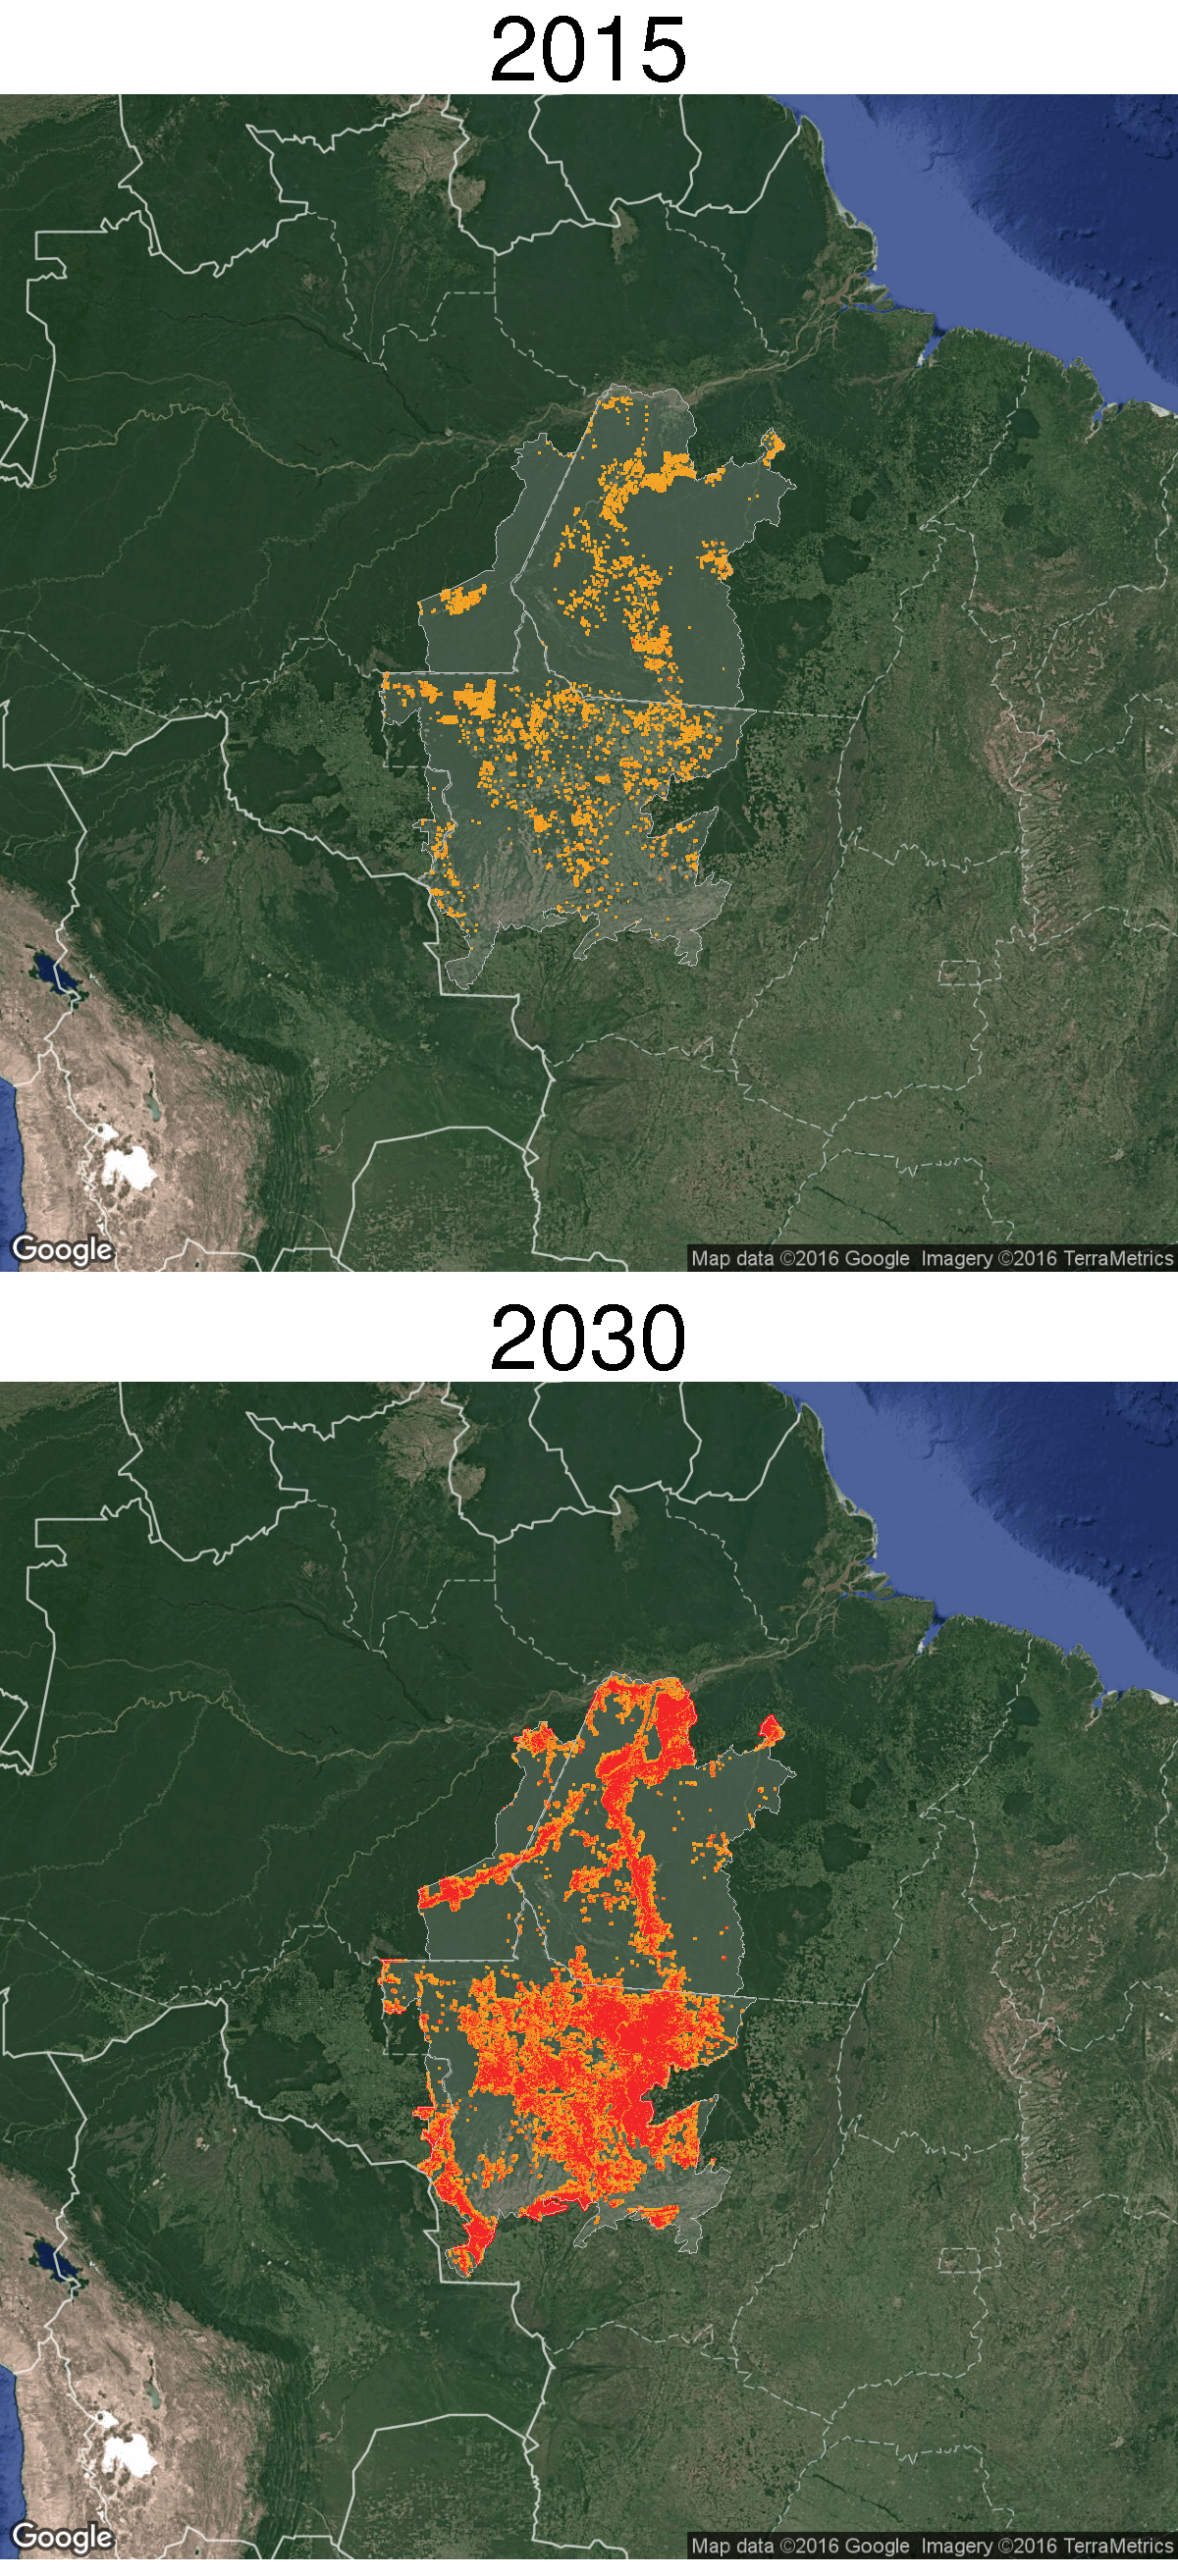
\includegraphics[width=.9\linewidth]{deforest_compare.pdf}
 \caption{Observado o desmatamento em 2015 e projetou o desmatamento em 2030 entre os munic\'{i}pios da bacia do rio Tapaj\'{o}s.}
  \label{fig:deforest}
\end{figure}

%------------------------------------------------



\section*{O Efeito do Desmatamento no Balan\c co H\'{i}drico Local e Regional}
A precipita\c c\~{a}o \'{e} dependente tanto do vapor de \'{a}gua que est\'{a} sendo transportado no sentido contr\'{a}rio do vento, quanto da endrada de vapor de \'{a}gua por meio da evapotranspira\c c\~{a}o (ET). Sabe-se que o desmatamento tem in\'umeros efeitos negativos no ciclo da \~{a}gua e na energia nos ecossistemas tropicais. 

Primeiramente, as pastagens e as planta\c c\~oes de gr\~{a}os absorvem menos energia solar e evaporam menos \'{a}gua do que as florestas, reduzindo de maneira dram\'{a}tica a quantidade de energia e \'{a}gua que s\~{a}o devolvidas \'{a} atmosfera. Ao privar a atmosfera de energia e \'{a}gua, ocorre uma diminui\c c\~{a}o das chuvas na regi\~{a}o \cite{coe2009influence}. Como resultado da remo\c c\~{a}o de \'{a}gua da atmosfera e de mudan\c cas do equilíbrio energ\'etico, prev\^{e}-se uma redu\c c\~{a}o das chuvas em escala local e regional, com consequ\^{e}ncias potencialmente negativas para a produ\c c\~{a}o de gr\~{a}os \cite{oliveira2013large}. Em seguida, devido \'as mudan\c cas na evapora\c c\~{a}o e nas chuvas, a vaz\~{a}o dos rios \'e alterada. A paisagem com floresta fornece uma libera\c c\~{a}o lenta de \'agua em c\'orregos durante a esta\c c\~{a}o seca. Uma paisagem desmatada pode resultar em grandes mudan\c cas sazonais da \'agua do rio, muitas vezes com muito mais na esta\c c\~{a}o chuvosa e muito menos na esta\c c\~{a}o seca. Estes tipos de altera\c c\~{o}es podem ser especialmente dif\'iceis para a gera\c c\~{a}o de energia hidrel\'etrica consistente e a mudan\c ca da fun\c c\~{a}o ecol\'ogica de rios e c\'orregos.

%------------------------------------------------

\section*{Nossa Pergunta}
Como o desmatamento na Bacia do Rio Tapaj\'{o}s afeta a variabilidade sazonal na vaz\~{a}o do rio, a ET e a energia líquida (potencial de precipita\c c\~{a}o)? A seguir foram utilizados os resultados de modelagem da superf\'icie terrestre (IBIS) para quantificar o efeito do desmatamento sobre a magnitude das mudan\c cas nas referidas caracter\'isticas do balan\c co h\'idrico.
%------------------------------------------------

\section*{Resultados e Recomenda\c c\~{a}oes}
Os resultados mostram que, com o atual nível de \'area desmatada na Bacia do Rio Tapaj\'os (34\%), a vaz\~{a}o do Rio Tapaj\'os \'e muito menor na esta\c c\~{a}o seca, enquanto que a ET \'e menor durante a esta\c c\~{a}o chuvosa. De maneira similar, a energia líquida total devolvida \'a atmosfera, um fator desencadeador de chuvas, \'e fortemente afetada pelo desmatamento. Sugerem-se as seguintes estrat\'egias pol\'iticas para evitar ou compensar esses efeitos:


\renewcommand{\labelitemi}{${\color{DarkGoldenrod}\bullet}$}
\begin{itemize}	
\item A constru\c c\~{a}o de hidrel\'etricas compromete o seu pr\'oprio potencial de produ\c c\~{a}o de energia se estiver associada ao desmatamento, devido \'a varia\c c\~{a}o da sazonalidade na gera\c c\~{a}o de \'agua. Prop\~oe-se a utiliza\c c\~{a}o de estrat\'egias alternativas de energia, a exemplo da energias solar e e\'olica, quando poss\'ivel, para manter o correto funcionamento do ciclo hidrol\'ogico.
\item O desmatamento numa \'area pode afetar a chuva a centenas de km de dist\^{a}ncia, alterando potencialmente a produ\c c\~{a}o de gr\~aos e os ecossistemas naturais. As pol\'iticas
para reduzir o desmatamento que est\~ao direta e indiretamente associadas \'a constru\c c\~{a}o de barragens, \'a redu\c c\~{a}o dos custos de recupera\c c\~{a}o florestal e incentivos \'a manuten\c c\~{a}o de \'areas florestais devem ser priorit\'arias.
\item Alguns dos custos de monitoramento, restaura\c c\~{a}o e prote\c c\~{a}o devem ser embutidos nos custos do governo para financiar a constru\c c\~{a}o desses projetos.
\end{itemize}


\begin{figure}[h]
\vspace{-3.5em}
  \includegraphics[width=1\linewidth]{SeasonalEffects.pdf}
\vspace{-2em}
 \caption{Consequ\^encias do desmatamento no volume de \'agua e na ET a cada m\^es, entre 200 e 2014. Se n\~ao houvesse consequ\^encias do desmatamento, as duas linhas seriam planas com uma raz\~ao de 1 ao longo dos meses. }
  \label{fig:deforest}
\vspace{-2em}
\end{figure}

\begin{figure}[h]
\vspace{-1em}
  \includegraphics[width=1\linewidth]{Rnet_rec.pdf}
\vspace{-2em}
 \caption{Diferença de energia l\'iquida (potencial de chuva) abaixo do limite legal em uma \'area desmatada (azul) e n\'ivel observado do desmatamento (vermelho). }
  \label{fig:deforest}
\end{figure}
 



%----------------------------------------------------------------------------------------


%----------------------------------------------------------------------------------------
%	REFERENCE LIST
%---------------------------------------------------------------------------------------- 
\vspace{-1em}
{\scriptsize \bibliography{reference}}

%{\bf \noindent Agradecimentos}\\
%{\small Agradecemos Isabel Silva do IPAM por acesso aos dados de desmatamento e resultados da simula\c c\~{a}o.} 
%----------------------------------------------------------------------------------------

\end{document}